\chapter{Relationship Extraction on CERED}
The goal of this part of the thesis is to train a relationship extraction model for the Czech language. To the best of our knowledge, there is no baseline for such a model, since there is no Czech relationship extraction datasets. In the first part of the thesis, we generated CERED, a family of relationship extraction models that we can use.

If we just trained the model on our dataset, we would be unable to determine, whether the model is well designed. We therefore adapt the model to be trainable both on Czech and on English. We assume that if the English version is competitive on popular English relationship extraction dataset, the Czech version is reasonably good.

In this chapter, we first describe the model, then we evaluate it on English datasets and lastly we report the results on CERED.

\section{Model}

We based our model on the BERT model described in the \autoref{sec:bert}. The model architecture is quite straightforward. The goal of the whole model is to predict a relation based on a given relation mention. We modify the input by adding several special tokens as we show in \autoref{obr:rose}. Then we use the tokenizer, which is attached to the specific BERT, and we feed the output of the tokenizer to the model. The model computes abstract representations of all input tokens. We concatenate the representations that correspond to some of the special tokens ([E1], [E2] and [CLS]). On top we apply a dropout layer and finally a dense layer which predicts the class. 

For Czech, we fine-tune the multilingual BERT, for English we fine-tune BERT\textsubscript{BASE}. We use the transformers library (\cite{Wolf2019HuggingFacesTS}) for BERT manipulation.



\begin{figure}[h]
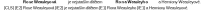
\includegraphics[width = 1\textwidth]{./img/rose}
\caption{Special tokens added for each mention. The sentence is a mention of \relation{father}{Ron Weasley}{Rose Weasley}. We add tokens to mark where each entity starts and ends. The [CLS] token is part of BERT input and was pre-trained to capture the whole input sequence via the NSP loss.}
\label{obr:rose}
\end{figure}



\section{Results}

We trained the model described in the previous section on the three English datasets introduced in \autoref{chap:datasets} and on CERED. We hoped for our model to be competitive with other models, that build on BERT. At the same time, we did not use any additional data for the training and we only used BERT base, because the multilingual BERT is not available in the large size. Therefore we do not expect to score as well as state-of-the-art results. We referred to results provided by nlpprogres\footnote{\url{http://nlpprogress.com/english/relationship_extraction.html}} when researching the scores achieved on each dataset.

We did not fine-tune the hyperparameters (such as the learning rate or dropout rate). 


\subsection{S10T8}

On S10T8 the model stopped training after 10 epochs (i.e. in less than 20 minutes on a singe GPU) and achieved  86.54\% in the official metric. The state-of-the-art result was achieved by \cite{baldini-soares-etal-2019-matching} with 89.5\%, we include more results in \autoref{table:S10T8results}.


\begin{table}[h]
\centering
\caption{Results on S10T8.}
\label{table:S10T8results}
\begin{tabular}{l c }
\hline
Paper/Source & F1 \\
\hline
\hline
Our model & 86.54 \\
\textbf{\cite{baldini-soares-etal-2019-matching}} & \textbf{89.5} \\
\textit{\cite{DBLP:journals/corr/abs-1905-08284}} & 89.25 \\
\textit{\cite{DBLP:journals/corr/abs-1901-08163}} & 85.2 \\
\hline

\end{tabular}
\end{table}


\subsection{TACRED}

Training on TACRED did not take much longer (4 epochs and under two hours). The state-of-the-art on this dataset was also achieved by \cite{baldini-soares-etal-2019-matching} with 71.5\% F1 (micro-averaged over instances with positive relationships). We scored 65.65, we include more results in \autoref{table:TACREDresults}


\begin{table}[h]
\centering
\caption{Results on TACRED.}
\label{table:TACREDresults}
\begin{tabular}{l c }
\hline
Paper/Source & F1 \\
\hline
\hline
Our model & 65.65 \\
\textbf{\cite{baldini-soares-etal-2019-matching}} & \textbf{71.5} \\
\textit{\cite{zhang-etal-2018-graph-TACRED}} & 68.2 \\
\textit{\cite{zhang-etal-2017-position_TACRED}} & 65.1 \\
\hline

\end{tabular}
\end{table}

\subsection{Riedel NYT}

Our model was unable to properly train on this dataset. It learns to always predict the negative relation (about 80\% of the dataset is the negative relation). The distribution of relations in the dataset itself is most likely not the main issue (since TACRED has a similar distribution of relations). It is an interesting open problem, why a straightforward BERT model does not work on this dataset, \cite{nyt-nefunguje} encounter similar (less severe) issues. However, our main goal was to provide a model for Czech, so we leave the investigation for future work.




\subsection{CERED}
We trained our model on all CERED versions. The performance of respective models was mostly as expected.  We pinpoint few things we observed in the results. 

We assume that the highest macro-F1 was achieved on CERED2 because we choose the relation inventory for CERED1-4 based on CERED2. CERED0 has a huge relation inventory and therefore it is not surprising that when weighting over classes, the metric is low.

The fact, that model trained on CERED4 preforms relatively well, shows, how remarkable BERTs (and the concept of pre-trained models) are for tasks with small datasets. The low macro-F1 on CERED4 can be explained quite easily. When we put constraints on which mentions will be kept in CERED4, we did not ensure, that the dataset will be balanced. In \autoref{obr:relations} we see, how imbalanced the dataset really is.





\begin{table}[h]

\caption{Results on CERED, we measured micro and macro F1 on the corresponding test sets for each version. Moreover, we measured the performance of models trained on CERED1-4 on CERED2 test set, to see the direct comparison.}

\label{table:CEREDsResults}

\begin{tabular}{p{2,3cm} r r r }

\hline
Dataset & \# micro-F1 & macro-F1 & micro-F1 on CERED2 test \\
\hline
\hline
CERED0 & 84.49 & 44.33 & -\\
CERED1 & 83.94 & 76.58 & 81.72 \\
CERED2 & 84.78 & 79.79 & 84.78 \\
CERED3 & 77.29 & 73.96 & 82.33 \\
CERED4 & 77.66 & 58.84 & 79.79 \\
\hline


\end{tabular}

\end{table}


